\documentclass[12pt]{article}
\usepackage[top=0.5in, right=0.5in, left=0.5in, bottom=0.5in]{geometry}
\usepackage{algorithm}
\usepackage[noend]{algpseudocode}
\usepackage{graphicx}
\graphicspath{ {./} }

\title{\textsc{Final}}
\author{Henry Trinh}

\begin{document}
\maketitle

\newpage
\section*{Problem 1}
\subsection*{Part A}
\textbf{True.} Given an undirected graph with edge weights that are all distinct(unique), there will only be
only one unique minimum spanning tree. Since there's only one possible MST in the scenario where a graph 
has all unique edge weights, both Prim's and Kruskal's algorithm will produce the same MST.

\subsection*{Part B}
\textbf{True.} Kruskal's algorithm utilizes a greedy approach to create a spanning tree that has the minimum cost by
taking in the current minimum available edge that doesn't create a cycle with the current tree. This greedy algorithm 
can be used with a decreasing order of weights for the same effect to get the spanning tree with maximum cost. 
\newline
\newline
Given an example of a tree with only negative edge weights, running Kruskal's algorithm will yield a spanning tree with minimum cost, which will be negative. 
However, if we now take the same ordering of edge weights, but apply an absolute value to every single weight, we will get a spanning tree with maximum
cost instead since before we had the most negative cost while now, we have the most positive cost.

\subsection*{Part C}
\textbf{False.} We can prove this by counter example.
Given the undirected graph depicted below with $n=4$ vertexes/nodes $\{A,\ B,\ C,\ D\} \in V$ which contains a negative cycle:
\newline
\begin{center}
    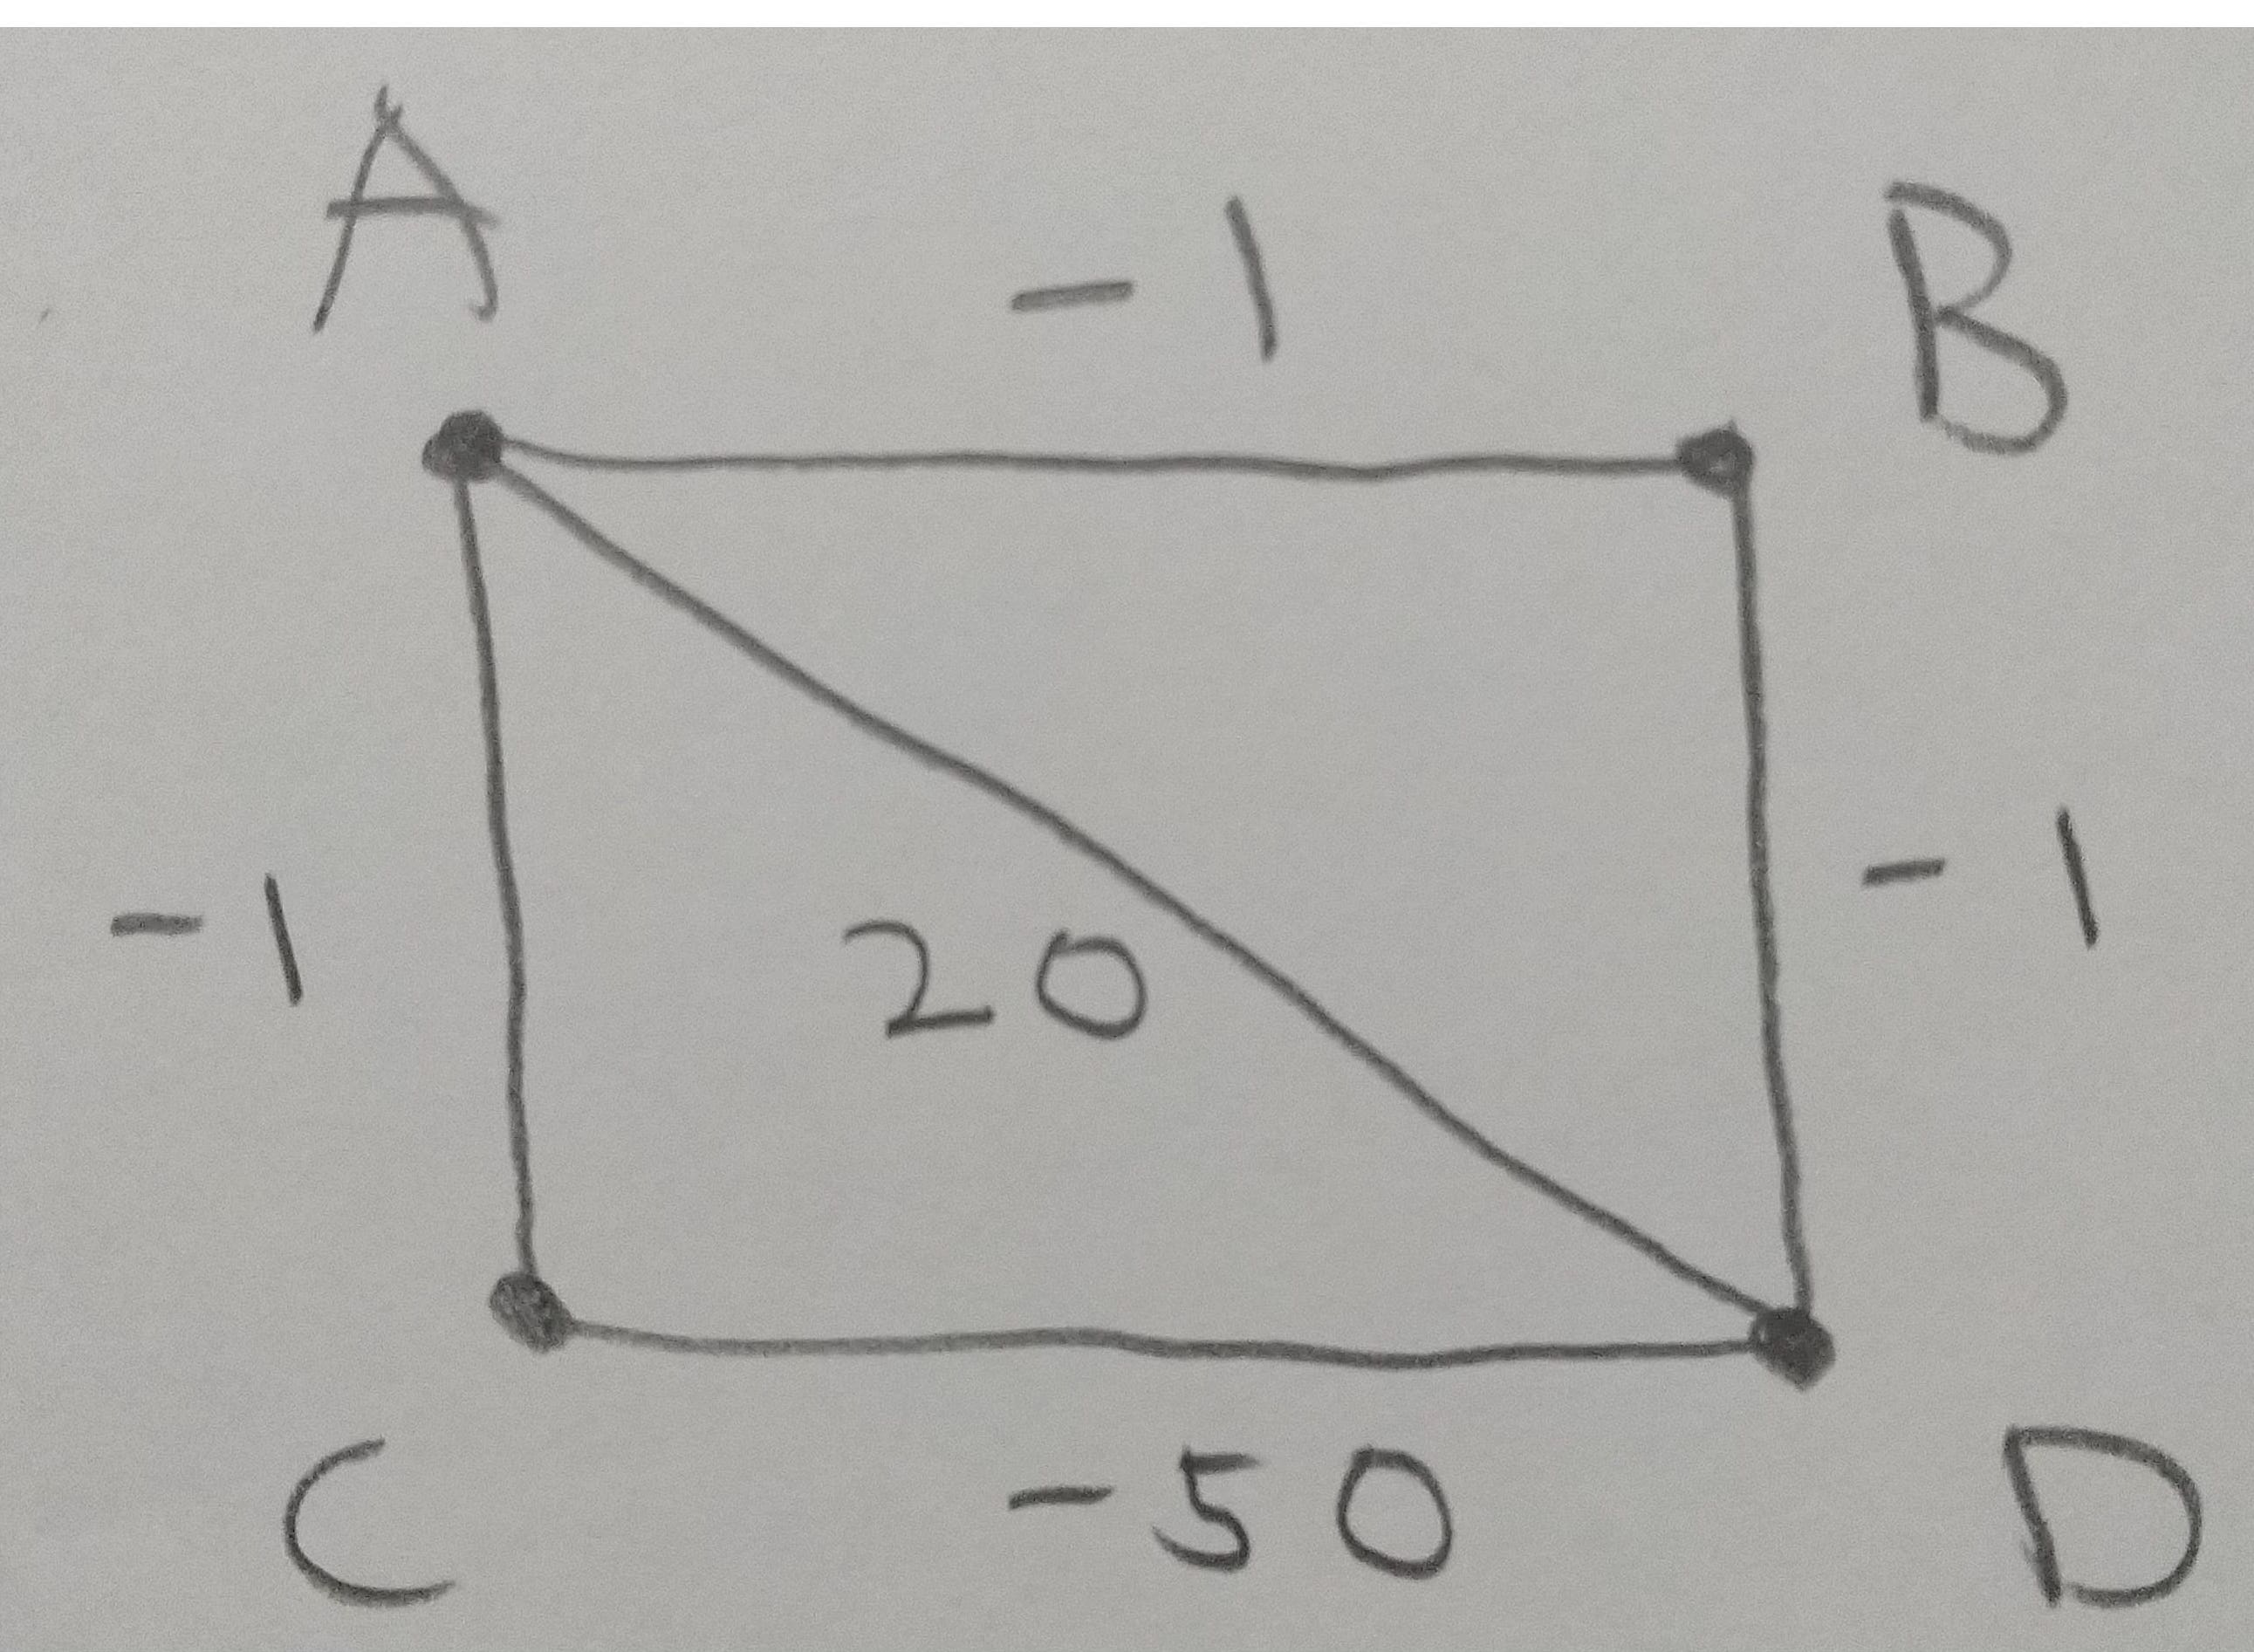
\includegraphics[scale=0.05, angle=0]{hi2.jpg}
\end{center}
Say that $s=A$ and $t=D$, where we have to find the shortest paths using $n$ and $n+1$ edges, we can see that the shortest path
with at most $n$ edges is $A->C->D->C->D$, which has a weight of $-1-50-50-50=-150$. The shortest path with at most $n+1$ edges is also $A->C->D->C->D$,
which has a weight of $-150$. Since the shortest path from $s$ to $t$ containing at most $n+1$ edges is NOT strictly shorter than the
shortest path containing at most $n$ edges $(-150==-150)$, we can say that by providing this counter example, the statement is false.

\subsection*{Part D}
\textbf{True.} This is a theorem (from class) where $P \leq_p NP$. Since $NP$ is more complex than $P$, we can always reduce an algorithm to something 
more complex.

\newpage
\section*{Problem 2}

Algorithm A: $O(n\log n)$
\newline
Algorithm B: $O(n^2)$
\newline
Algorithm C: $O(n^2)$
\newline
\newline
Algorithm A is the fastest algorithm.
\begin{center}
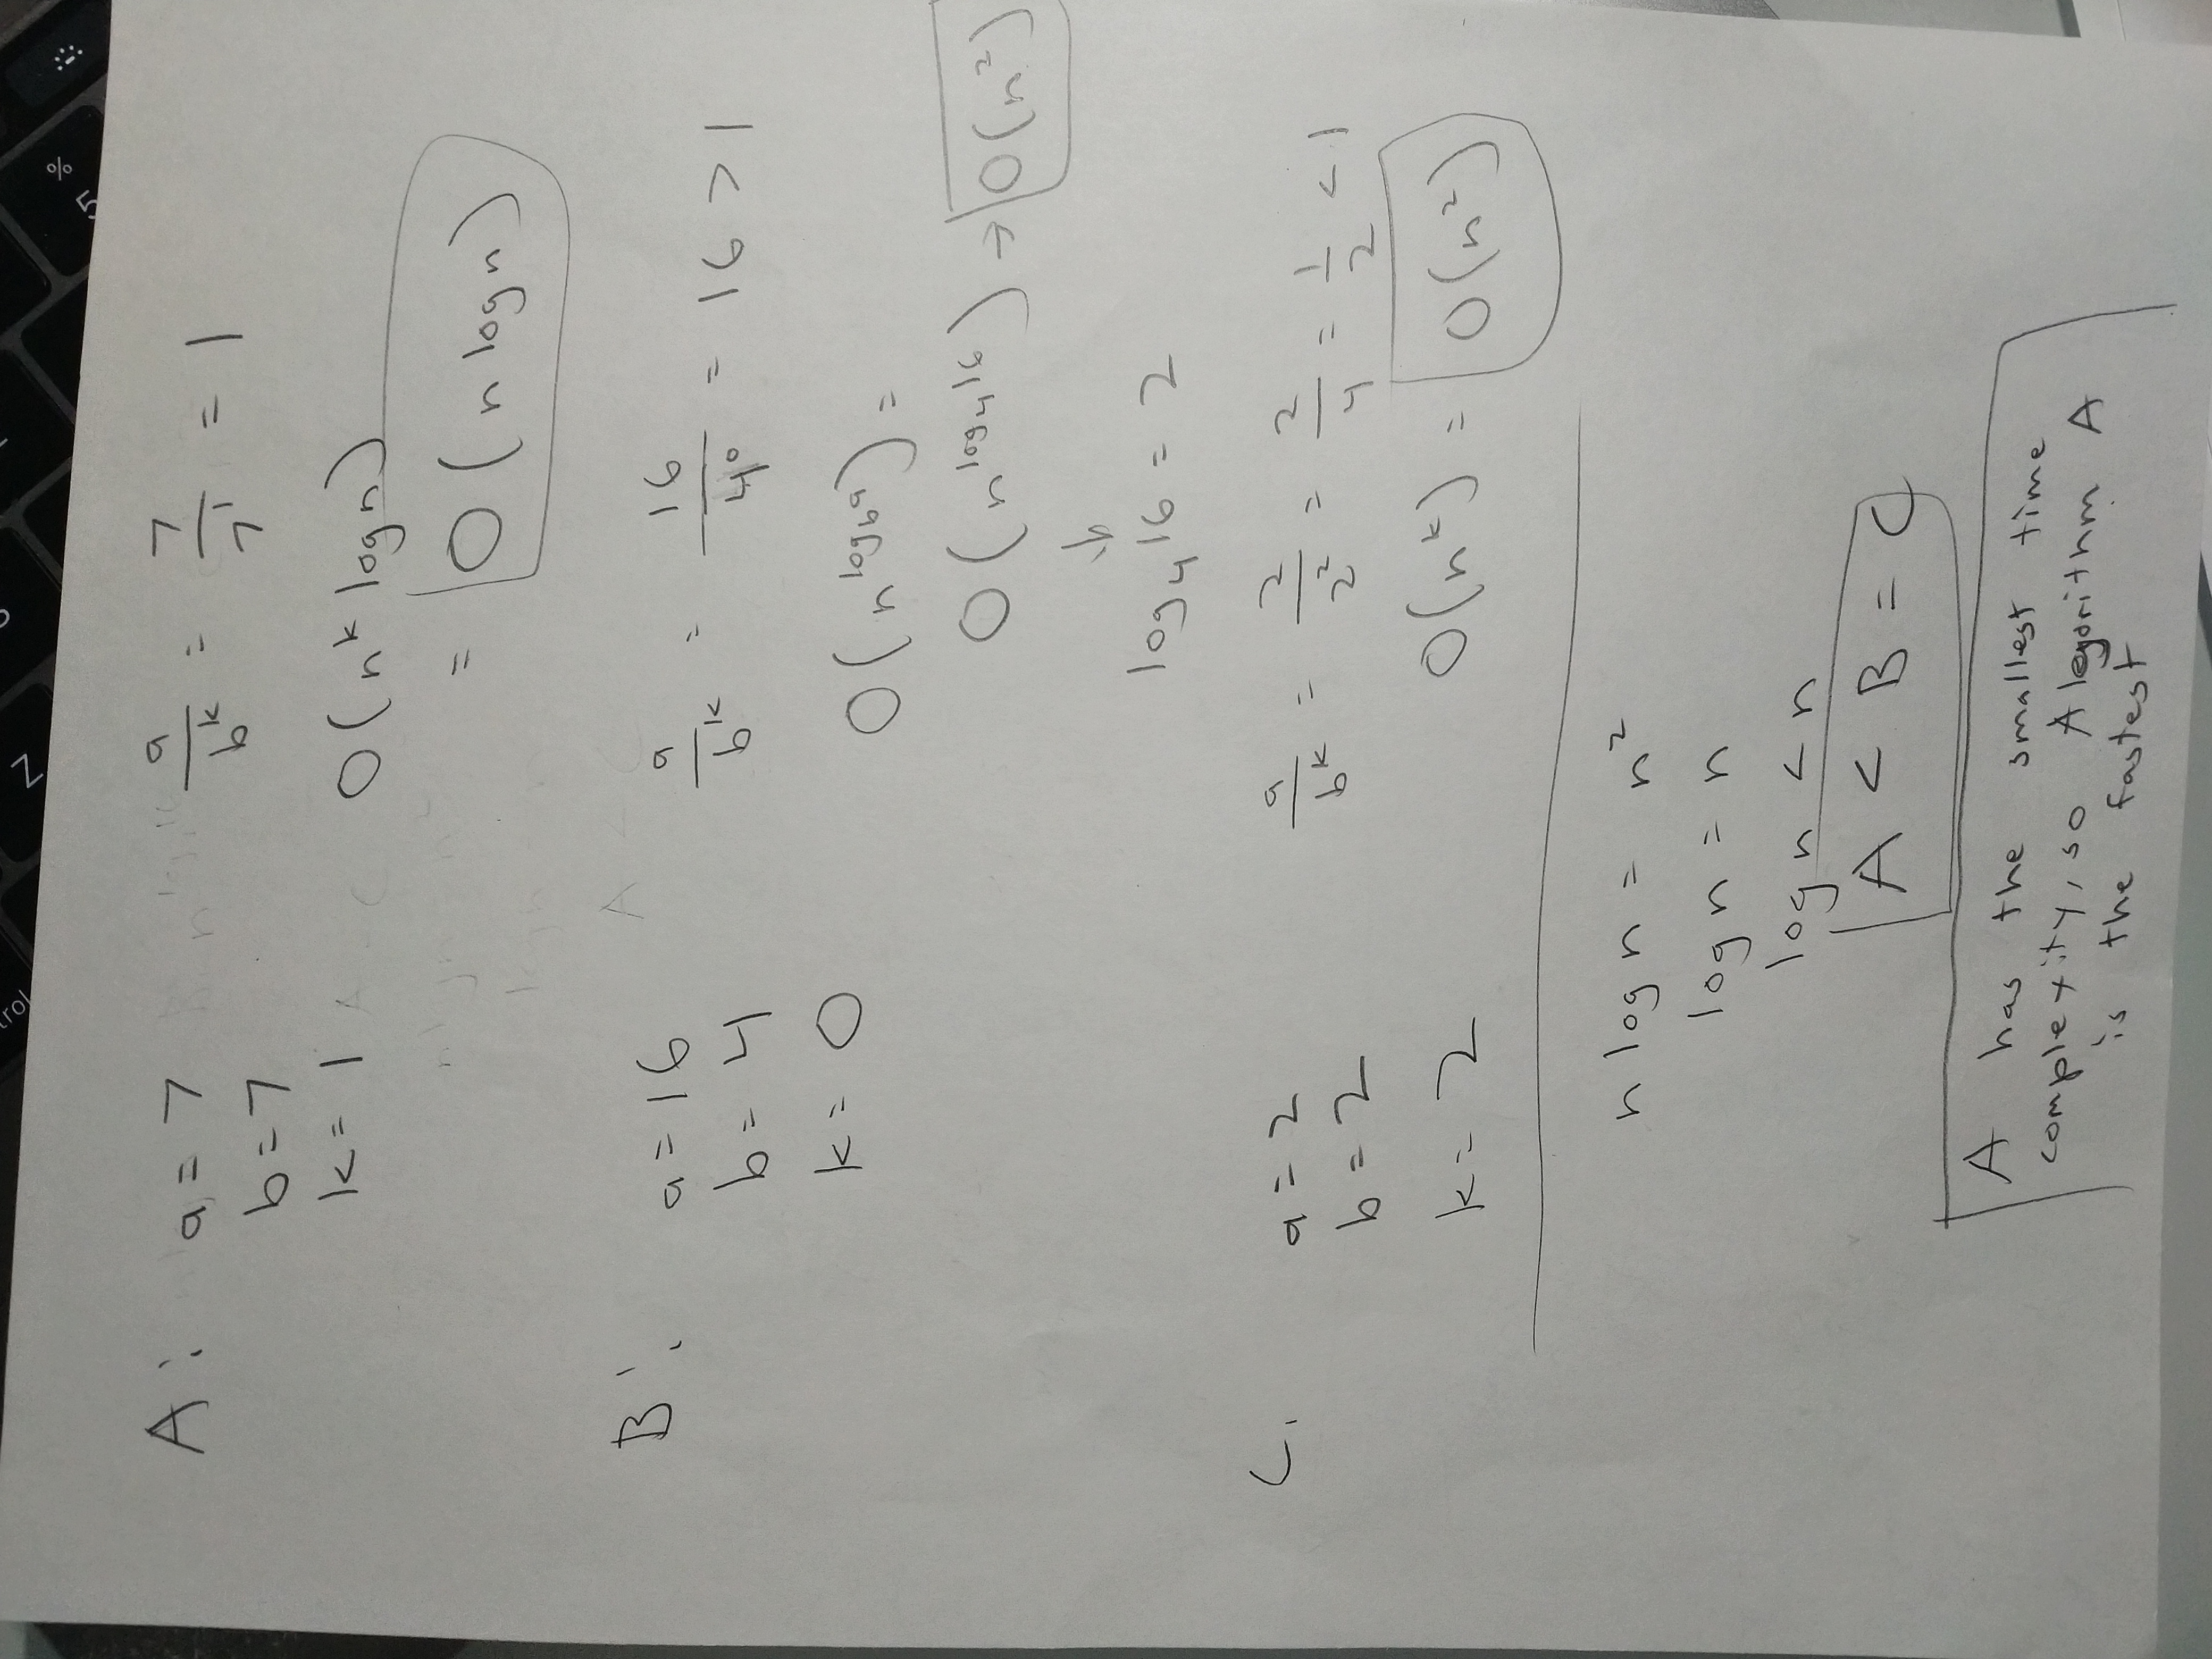
\includegraphics[scale=0.14, angle=270]{hi.jpg}
\end{center}

\newpage
\section*{Problem 3}
\begin{algorithm}
\caption{Partition elements in an array based on values}
\begin{algorithmic}[1]
\State $arr \gets $ array with $n$ integers
\State $partitions \gets $ empty array
\For {$i$ in the range of $0...n-1$}
    \State $currUnion \gets$ subset of elements in $arr$ whose indexes are in a set in $partitions$
    \State add $arr[i]$ to $currUnion$
    \If {$query(currUnion) == length(partitions) + 1$}
        \State $newSet \gets $ initialize new set with $i$
        \State append $newSet$ onto $partitions$
        \State continue
    \EndIf
    \State
    \State $left \gets 0$
    \State $right \gets length(partitions) - 1$
    \While {$left <= right$}
        \State $mid \gets left + (right - left) / 2$
        \State
        \State $midPart \gets $ subset of elements in $arr$ whose indexes are in $partitions[mid]$
        \State add $arr[i]$ to $midPart$ 
        \If {$query(midPart) == 1$}
            \State add $i$ to $partitions[mid]$
            \State break
        \EndIf
        \State
        \State $leftParts \gets $ all sets in $partitions$ from index 0 to index $mid - 1$
        \State $leftUnion \gets $ subset of elements in $arr$ whose indexes are in a set in $leftParts$
        \State add $arr[i]$ to $leftUnion$
        \If {$query(leftUnion) == length(leftParts)$}
            \State $right \gets mid - 1$
        \Else
            \State $left \gets mid + 1$
        \EndIf 
    \EndWhile
\EndFor
\State return $partitions$
\end{algorithmic}
\end{algorithm}
\noindent
This algorithm utilizes a binary search for each element in the given array. To explain further,
we utilize an array of sets, $partitions$, where the sets will contain elements from the given array, to store 
our partitions. 
\newline
\newline
For every element in the given array, we have two cases. The first case is that the current
element is unique and does not belong to any set in $partitions$. We do this by querying all the elements whose indexes are in 
$partitions$ along with the current element and checking to see if the output of the query is equal to the length
of $partitions$. If it is not equal, that means our current element is unique and we just create a new set with the 
current element's index and add that set to $partitions$. The second case is that the output of the query is equal to the
length of $partitions$. In this case, that means that our current element belongs to a set in $partitions$ and
we need to find this set. We can do this utilizing a binary search method to bring our search time complexity from 
linear to logarithmic. To do this, we query just the elements whose indexes are in the middle set of $partitions$, add the current element, and check the output against the number $1$.
If it's $1$, the element belongs to that set. If not, we continue a binary search. We can decide which half of $partitions$ to
search by querying one of the halves to check if it belongs in that set and continue until we find the set that the current
element belongs to.
\newline
\newline
This algorithm utilizes $O(n\log{n})$ queries because we utilize a binary search that uses the $query$ to power its search.
Since a binary search has a time complexity of $O(\log n)$, each binary search would use $O(\log n)$ queries as well. 
We are perfoming this binary search on every element in the array. Since we perform the binary search $n$ times, this algorithm 
partitions all elements into sets in $O(n\log n)$ queries.

\newpage
\section*{Problem 4}
\subsection*{Part A}
The optimal policy is where $S_1=\{c_1,\ c_2,...,\ c_{n/2}\}$ and $S_2=\{c_{n/2 + 1},...,\ c_n\}$.
This is such that each set $S_1$ and $S_2$ each have $n/2$ cells for $n$ cells. We can derive
this using calculus.
\newline
\newline
Given the variable $x$, which represents the number of cells in $S_1$, we can derive that the expected
number of activations is $x + (n-x)(1-(x/n))$. Taking the derivative of the function in respect to $x$,
we obtain the derivative $n-x+(x^2/n)$ to find the value of $x$ that would minimize the value of our number 
of activations. This would be solved to $x=n/2$, which means that having half the cells in each set would give the least expected number
of activations. This would be most optimal.

\subsection*{Part B}
We can prove that an in an optimal policy, $S_1$ is a set of cells which is the prefix of the decreasing
order of the cells according to their probabilities by proving by contradiction.
\newline
\newline
Given that in an optimal policy, our $S_1$ is the prefix of an increasing order of cells based on thier probabilities. In this problem, each slot's 
number of activations depends on the sum probabilities of the cells used before the current slot subtracted
from 1. Say we flip the order of the cells so that it is in decreasing order instead of increasing. With the 
same number of cells in each policy. Our first slot's number of activations would stay the same. However, 
each policy thereafter would have its number of activations decrease since the sum of probabilities subtracted 
from 1 in each slot would be larger than its counterpart in our optimal policy. This is a contradiction since our newly 
formed policy would have a smaller number of activations than our optimal policy, which means that our optimal policy 
is not optimal and that an optimal policy would have $S_1$ contain the prefix of the decreasing order of cells based 
on their probabilities.

\newpage
\subsection*{Problem 4 Part C}
\begin{algorithm}
\caption{Calculate optimal policy}
\begin{algorithmic}[1]
\State $d \gets $ slots
\State $p \gets $ probabilities of cells
\State $c \gets $ cells
\State $n \gets $ length of $c$
\State $orderC \gets $ sort $c$ in decreasing order based on $p$
\State $orderP \gets $ sort $p$ in decreasing order
\State $psums \gets $ sum of $orderP$ for each index up to and including that current index
\State
\State $dp \gets $ 2d array of size $n$ x $d$
\State $traceArr \gets $ 2d array of size $n$ x $d$ initialized with all 0's
\State $S \gets $array initialized with $d$ empty sets
\State
\State set first row values of $dp$ to be all $1$
\For{$i=0;i<n;i++$ }
    \State $dp[i][0] = i + 1$
\EndFor
\State
\For{$i=1;\ i < n;\ i++$}
    \For{$j=1;\ j < d;\ j++$}
        \State $curr \gets \infty$
        \State $lastSplit \gets 0$
        \For {$k = 0;\ k \leq i;\ k++$}
            \State $temp \gets dp[k][j-1] + (i-k) * (1-psums[k])$ 
            \If {$temp < curr$}
                \State $curr \gets temp$
                \State $lastSplit \gets k$
            \EndIf
        \EndFor
        \State $traceArr[i][j] \gets lastSplit$
        \State $dp[i][j] \gets curr$
    \EndFor
\EndFor
\State $row \gets n - 1$
\For{$j=d-1;\ d > 0;\ d--$}
    \State $split \gets traceArr[row][j]$
    \For{$i=split + 1;\ i \leq row;\ i++$}
        \State add $orderC[i]$ to $S[j]$
    \EndFor
    \State $row \gets split$
\EndFor
\ForAll {$i$ in range $0...row$}
    \State add $orderC[i]$ to $S[0]$
\EndFor
\State return $dp[n-1][d-1],\ S$
\end{algorithmic}
\end{algorithm}
\noindent
This algorithm works by using a bottom-up dynamic programming approach utilizing a 2D array $dp$ of size 
$n$ x $d$, where $n$ is the number of cells and $d$ are the number of slots. In this problem, we proved
in Part B that the policy order is dependent on the decreasing order of the probabilities of the cells.
We can first sort the cells based on the decreasing probabilities into an array $orderC$ and we store those 
sorted probabilities in $orderP$. In our base cases, we can safely assume that the entire first row of the
$dp$ is 1 since there would only be 1 cell at this time. We can also assume that the entire first column 
of $dp$ is the increasing index starting at 1. This is because as you put cells into the first slot, the 
number of activations just increases with how many cells are in that first slot. We also note that we can
initialize another 2D array $traceArr$ with the same dimensions as $dp$, where all of its values are initialized
to 0. We also initialize a helper array that sums up all of the ordered probabilies up to the current index.
\newline
\newline
After filling out these base cases, we can proceed to fill out the array. At each coordinate of $dp$, we have 
to calculate the number of activations up to the current row we are on and take the minimum number of activations.
To do this, we can refer to all the previous rows of the previous slot. These are the values at which the optimal 
number of activations is set at. For each of these values, we calculate the activations of a slice taken from 
that previous row up to the current row we are at. This can be calculated as the number of cells in the slice 
multiplied to the output from subtracting the sum of probabilities up to the previous row from 1. We add this 
calculation to the value we are currently at in the previous column. To find the optimal number of activations
for our current coordinates, we just take the minimum of these calculations. We also store which row provided us 
the minimum number of activations for our current row and store the row value into $traceArr$. By the end of this,
the optimum number of activations is provided at the last row and last column of $dp$.
\newline
\newline
We also trace how our policy is made to get the optimal number of activations using our filled out $traceArr$. We 
will store our policy in an array of sets $S$. Starting from the last row and last column. We take the value 
at $traceArr[row][col]$. This value we get is the last row/cell of the previous slot. We will then proceed to add 
the corresponding cells starting from the value up to and including our current row according to $orderC$ to 
the corresponding slot in $S$. We continue this method until we finish the first slot. In essence, this method
fills out the policy starting from the last slot.
\newline
\newline
This algorithm has a runtime of $O(d * n^2)$ where $n$ is the number of cells and $d$ is the number of slots because 
the main driving body of our algorithm iterates through the number of slots for each cell. In each of these, we also
traverse the number of cells again. All the other functions in our algorithm are at most linear time complexity, adding
no effect to the algorithm's time complexity. This algorithm is in polynomial time, satisfying the requirements.

\newpage
\section*{Problem 5}
\vspace*{-1.5em}
\begin{algorithm}
\caption{Minimum possible wasted area}
\begin{algorithmic}[1]
\State $W \gets $width of given rectangle
\State $L \gets $length of given rectangle
\State $K \gets$ number of shapes
\State $a \gets $ array of width of shapes -> should be length $K$
\State $b \gets $ array of length of shapes -> should be length $K$
\State $dp \gets$ 2D array of size $L + 1$ x $W + 1$ initialized with all 0's
\State 
\For {$i = 1;\ i \leq L;\ i++$}
    \For {$j = 1;\ j \leq W;\ j++$}
        \State $currWaste \gets i * j$
        \For{$k=0;\ k < K;\ k++$}
            \State $currA \gets a[k]$
            \State $currB \gets b[k]$
            \State
            \If {$currA > j$ or $currB > i$}
                \State continue
            \EndIf
            \If {$currA == j$ or $currB == i$}
                \State $currWaste \gets 0$
                \State break
            \EndIf
            \State
            \State $wasteHorz \gets dp[currB][j - currA] + dp[i - currB][j]$
            \State $wasteVert \gets dp[i - currB][currA] + dp[i][j - currA]$
            \State $currWaste \gets min(currWaste,\ wasteHorz,\ wasteVert)$
        \EndFor
        \State $dp[i][j] \gets currWaste$
    \EndFor
\EndFor
\State return $dp[L][W]$
\end{algorithmic}
\end{algorithm}
\noindent
This algorithm utilizes a bottom up dynamic programming approach by keeping a 2D array the size of 
rectangle to mimic it. Each cell of the array contains the minimum waste size of a rectangle of the 
size that the cell's coordinates makes. We can initialize the first row and column as all 0's because 
anything with a width or height of 0 has 0 area, and therefore can only have 0 waste. This approach 
works by building up smaller rectangles to eventually get to the largest one, which is of size $W$ x $L$.
For each cell, we must iterate through all the given shapes. Filling out the 2D array will yield us the 
smallest waste area at $dp[L][W]$
\newline
\newline
There are three cases that happens for each 
shape. The first case is if the shape does not fit in rectangle, at which point we disregard the shape
and move to the next. If the shape has the exact dimensions as the rectangle at the current cell, we 
know that the waste is 0 and we can move onto the next cell. The third case is if the rectangle can fit
inside of the current rectangle defined by the current cell's coordinates. In this problem, you can only 
create horizontal and vertical slices. For each type of slice defined by the current shape, we are given 
two smaller rectangles, which we would have solved already since the dimensions are smaller than our current 
dimensions. We can calculate the amount of waste area for each type of slice we would make and take the minimum 
of the horizontal slice waste, vertical slice waste, and the current waste we are keeping track of for the
current cell. 
\newline
\newline
This algorithm has a time complexity of $O(W * L * K)$ since there is one main driving loop with two nested 
loops. Each loop has a time complexity of $W$, $W$, $K$. This algorithm has polynomial time complexity.

\newpage
\section*{Problem 6}
We can start proving that Approx-3SAT is NP-Complete by proving that it is in NP. To do this we can 
prove that we can verify the solution to Approx-3SAT in polynomial time. This is possible by iterating through 
each clause and seeing that there are no duplicate literals as well as the clause being true. We can
then keep a counter to see if the solution satisfies at least n-1 clauses.
\newline
\newline
Given a boolean expression,$E$, which is the input of 3SAT and satisfies $n$ clauses,  we will try to create $E^\prime$ such that it has more clauses than $E$, but satisfies $n + 1$ clauses. 
Given any arbritrary $x_1$, $x_2$, $x_3$ and their negations, we can create 8 unique clauses using all combinations, where one clause is guaranteed to be false because there is only one combination
that gives all falses in a clause to make the clause false. We obtain $E^\prime$ which has $n^\prime = n + 8$.
\newline
\newline
Since 3SAT is NP-Hard, we can do a polynomial time reduction to Approx-3SAT. Using $E^\prime$ as an input, we can show that if $E$ can satisfy 
3SAT with an assignment, then $E^\prime$ also satisfies Approx-3SAT. Assuming that there is an assignment $E$ that satisfies 3SAT, then 
$n + 1 == n^\prime - 7$, where $n^\prime$ is the number of clauses in $E^\prime$. This means since one of the two extra clauses are true, 
all the original $n$ clauses from $E$ are also true.
\newline
\newline
This reduction from 3SAT can show that Approx-3SAT is NP-Complete.
\end{document} 